% checkpoint_presentation.tex
% Customer Segmentation for an Italian Fashion Retailer
% Intermediate Checkpoint Presentation — LUISS Data Science in Action 2025/26
%
% Compile: pdflatex checkpoint_presentation.tex  (run twice for page numbers)
%          or: latexmk -pdf checkpoint_presentation.tex

\documentclass[aspectratio=169,10pt]{beamer}

% ── Theme ─────────────────────────────────────────────────────────────────────
\usetheme{default}
\usefonttheme{structurebold}
\usepackage[T1]{fontenc}
\usepackage[utf8]{inputenc}
\usepackage{booktabs}
\usepackage{graphicx}
\usepackage{amsmath}
\usepackage{eurosym}

% ── Colour scheme (matches technical_report.tex) ──────────────────────────────
\definecolor{navy}{HTML}{1a1a2e}
\definecolor{accent}{HTML}{4361ee}

\setbeamercolor{title}{bg=navy, fg=white}
\setbeamercolor{subtitle}{fg=white}
\setbeamercolor{author}{fg=white}
\setbeamercolor{institute}{fg=white!85}
\setbeamercolor{date}{fg=white!85}
\setbeamercolor{frametitle}{bg=navy, fg=white}
\setbeamercolor{structure}{fg=accent}
\setbeamercolor{block title}{bg=accent!15, fg=navy}
\setbeamercolor{block body}{bg=accent!5, fg=black}
\setbeamertemplate{navigation symbols}{}
\setbeamertemplate{footline}{%
  \hfill\color{navy}\footnotesize\insertframenumber/\inserttotalframenumber%
  \hspace{6pt}\vspace{4pt}}

% ── Metadata ──────────────────────────────────────────────────────────────────
\title{The Hexagon\\\large Customer Segmentation for an Italian Fashion Retailer}
\subtitle{Intermediate Checkpoint Presentation}
\author{%
  \textbf{$\langle$Member~1 --- delegate$\rangle$} \quad \textbf{$\langle$Member~2$\rangle$}\\[2pt]
  \textbf{$\langle$Member~3$\rangle$} \quad \textbf{$\langle$Member~4$\rangle$}%
}
\institute{LUISS Guido Carli $\cdot$ Data Science in Action A.Y.\ 2025/26\\
  in partnership with \textbf{Jakala S.p.A.}}
\date{February 2026}

% =============================================================================
\begin{document}

% --- 1. Title slide -----------------------------------------------------------
\begin{frame}[plain]
\titlepage
\end{frame}

% --- 2. Agenda ----------------------------------------------------------------
\begin{frame}{Agenda}
\tableofcontents[hideallsubsections]
\end{frame}

% =============================================================================
\section{Business Context}
% =============================================================================

\begin{frame}{The Challenge: One Strategy for All Customers}
\begin{columns}[T]
  \begin{column}{0.53\textwidth}
    \textbf{The retailer today}
    \begin{itemize}
      \item 21{,}424 customers \,$\cdot$\, 24 months of data
      \item \euro12{,}084{,}646 observed revenue
      \item \textbf{Uniform campaigns}: same discount and messaging\\
            for every customer, regardless of value or behaviour
    \end{itemize}
    \vspace{0.5em}
    \textbf{Our hypothesis}\\
    Uniformity misallocates spend: VIP clients under-served, promotional
    buyers erode margins, lapsed buyers go unreactivated.
  \end{column}
  \begin{column}{0.44\textwidth}
    \begin{block}{Research Questions}
    \small
      \textbf{RQ1.} Can ML find distinct, interpretable segments\\
        from transactional data?\\[5pt]
      \textbf{RQ2.} What CRM strategies do they prescribe?\\[5pt]
      \textbf{RQ3.} What is the financial case for\\
        differentiated marketing?
    \end{block}
  \end{column}
\end{columns}
\end{frame}

% =============================================================================
\section{Data \& EDA}
% =============================================================================

\begin{frame}{Four Integrated Data Sources}
\centering\small
\begin{tabular}{@{}lrp{3.2cm}p{5.2cm}@{}}
\toprule
\textbf{Source} & \textbf{Rows} & \textbf{Key fields} & \textbf{Role} \\
\midrule
Anagraphics  & 21{,}480  & gender, DOB, province         & Demographic descriptors \\[2pt]
Transactions & 102{,}655 & date, store, amount, return   & Core behavioural signal \\[2pt]
Products     & ---       & product\_id, category         & Category affinity mapping \\[2pt]
Marketing    & ---       & email opened/clicked          & Digital engagement features \\
\bottomrule
\end{tabular}

\vspace{0.8em}
\begin{columns}[c]
  \begin{column}{0.3\textwidth}\centering
    \textbf{6.9\%} return rate\\{\footnotesize across all transactions}
  \end{column}
  \begin{column}{0.3\textwidth}\centering
    \textbf{Top 20\%} customers\\{\footnotesize drive $\sim$51\% of revenue}
  \end{column}
  \begin{column}{0.3\textwidth}\centering
    \textbf{Strong seasonality}\\{\footnotesize Nov--Dec peak each year}
  \end{column}
\end{columns}
\end{frame}

% =============================================================================
\section{Methodology}
% =============================================================================

\begin{frame}{Feature Engineering: 24-Variable Behavioural Matrix}
\begin{columns}[T]
  \begin{column}{0.48\textwidth}
    \textbf{RFM core (3)}\\
    recency, frequency, net monetary value\\[6pt]
    \textbf{Purchase behaviour (9)}
    \begin{itemize}\small
      \item Return rate, avg basket size, inter-purchase gap
      \item Seasonal concentration, multi-store flag, \ldots
    \end{itemize}
    \vspace{0.4em}
    \textbf{Preprocessing}
    \begin{itemize}\small
      \item 99\textsuperscript{th}-percentile winsorisation
      \item RobustScaler (median/IQR, outlier-robust)
    \end{itemize}
  \end{column}
  \begin{column}{0.48\textwidth}
    \textbf{Category affinity (6)}
    \begin{itemize}\small
      \item Share of wallet per macro-category
    \end{itemize}
    \vspace{0.4em}
    \textbf{Email engagement (6)}
    \begin{itemize}\small
      \item Open rate, CTR, recency of last click,\\
            newsletter subscription flag, \ldots
    \end{itemize}
    \vspace{0.4em}
    \begin{block}{Why not PCA?}
    \small UMAP preserves non-linear local structure better suited
    to behavioural manifolds than linear PCA.
    \end{block}
  \end{column}
\end{columns}
\end{frame}

\begin{frame}{UMAP + GMM Pipeline}
\centering
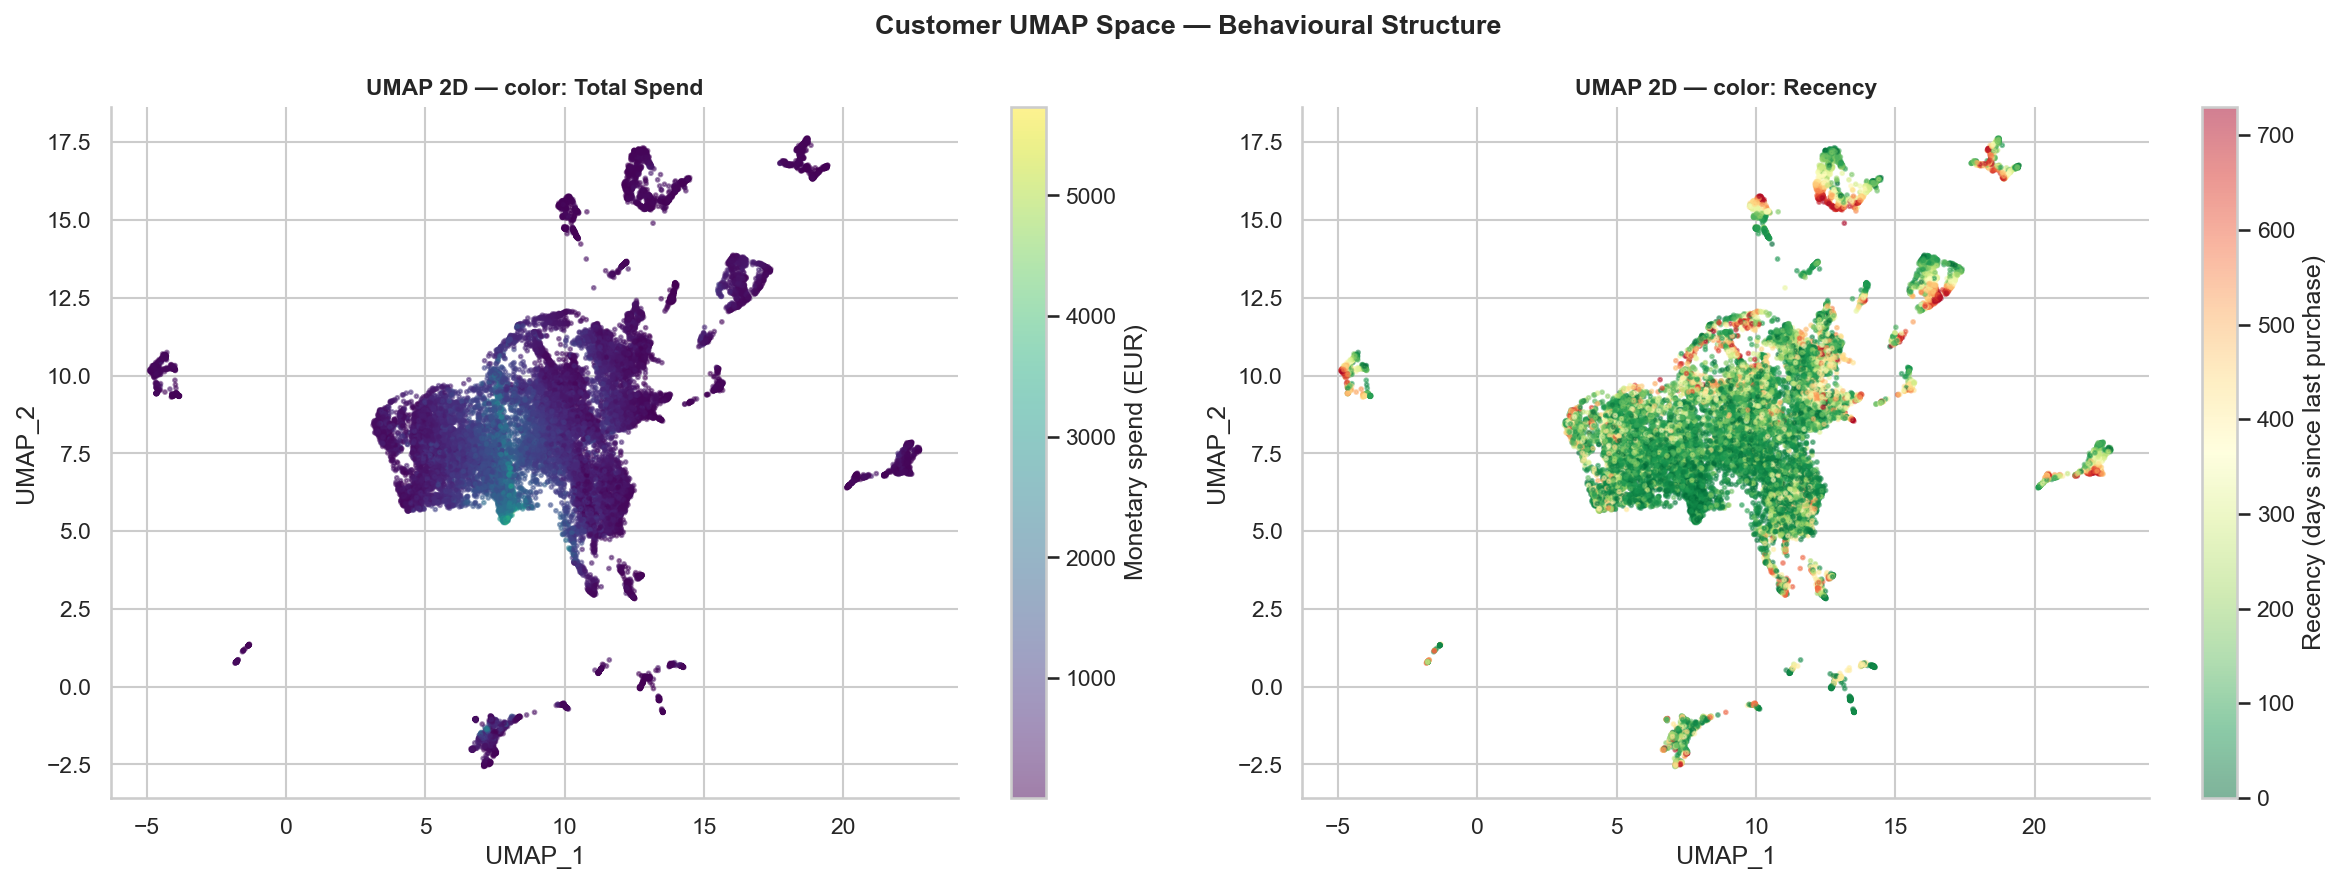
\includegraphics[width=0.80\textwidth]{assets/umap_space.png}

\vspace{0.5em}
{\small
  \textbf{Step 1.}\ RobustScaler
  $\;\rightarrow\;$ \textbf{Step 2.}\ UMAP 3D (n\_neighbors=30, min\_dist=0.1)
  $\;\rightarrow\;$ \textbf{Step 3.}\ GMM K=6 (full covariance, 10 inits, seed=42)
}
\end{frame}

% =============================================================================
\section{K Selection}
% =============================================================================

\begin{frame}{Why K\,=\,6? Four Convergent Criteria}
\begin{columns}[T]
  \begin{column}{0.46\textwidth}
    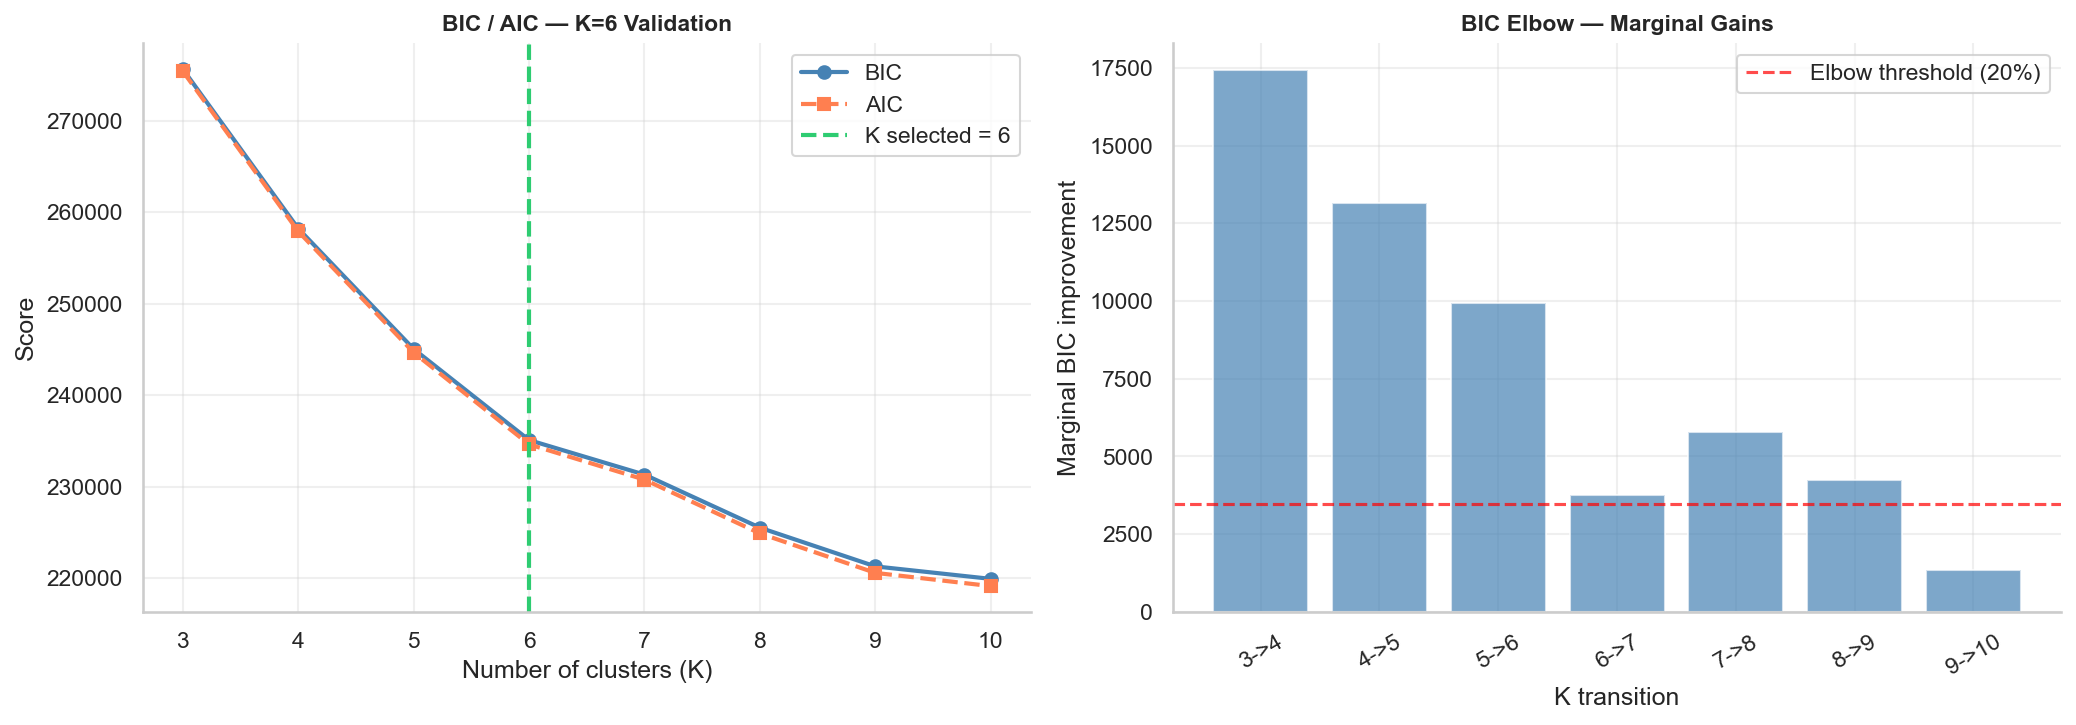
\includegraphics[width=\linewidth]{assets/bic_selection.png}
  \end{column}
  \begin{column}{0.51\textwidth}
    \begin{enumerate}\small
      \item \textbf{BIC elbow at K=6$\to$7}\\
            Absolute BIC min is K=10 but the marginal gain\\
            crosses the 20\% threshold at K=6$\to$7.\\[4pt]
      \item \textbf{Silhouette plateau, not peak}\\
            K=5: 0.388$\pm$0.004; K=6: 0.420$\pm$0.004;\\
            K=7: 0.450$\pm$0.003 (bootstrap, n=30).\\[4pt]
      \item \textbf{ARI partition stability}\\
            ARI(5,6)=0.892, ARI(6,7)=0.837, ARI(8,9)=0.716.\\
            K=6 sits in the stable region; collapse $\geq$K=8.\\[4pt]
      \item \textbf{GMM posterior stability}\\
            96.5\% posterior $>$0.80 (avg 0.983);\\
            collapses to 78\% at K=10.
    \end{enumerate}
    \vspace{0.3em}
    {\footnotesize\textit{Operational tie-breaker (secondary only):}
    budget cap of 6 simultaneous campaigns.}
  \end{column}
\end{columns}
\end{frame}

% =============================================================================
\section{Preliminary Results}
% =============================================================================

\begin{frame}{Six Segments: Preliminary Profiles}
\centering\small
\begin{tabular}{@{}lrrp{5.8cm}@{}}
\toprule
\textbf{Label} & \textbf{Size} & \textbf{Monetary (\euro)} & \textbf{Key characteristic} \\
\midrule
Active Loyalists   & 6{,}495  & 957 & Recent (131d), freq 5.0/24mo, broad cats \\[2pt]
Core Customers     & 10{,}256 & 484 & Mid-frequency, mid-tenure feeder pool    \\[2pt]
One-Shot Shoppers  & 2{,}727  & 115 & Recency 305d, freq 1.18, single-category \\[2pt]
Promo-Engaged      & 768      & 341 & Engagement 0.83 vs.\ avg 0.23 (3.7$\times$) \\[2pt]
Lapsed Low-Value   & 675      & 148 & Recency 315d, freq 1.10, reactivation candidate \\[2pt]
Churned            & 503      & 128 & Recency 306d, freq 1.04, smallest cluster \\
\bottomrule
\end{tabular}

\vspace{0.5em}
\begin{block}{Internal Validation (K\,=\,6 GMM on 3D UMAP, $n=21{,}424$)}
\centering\small
Silhouette: \textbf{0.419} \;$\cdot$\;
Davies--Bouldin: \textbf{0.760} \;$\cdot$\;
Calinski--Harabasz: \textbf{10,975} \;$\cdot$\;
GMM confidence (avg): \textbf{0.983}
\end{block}
\end{frame}

% =============================================================================
\section{Open Questions}
% =============================================================================

\begin{frame}{Questions for Jakala \& Next Steps}
\begin{columns}[T]
  \begin{column}{0.48\textwidth}
    \textbf{We'd like your input on:}
    \begin{enumerate}\small
      \item Are 6 segments operationally executable, or should we
            collapse the dormant tail into a single audience?
      \item Which behavioural feature(s) would Jakala's CRM team weight
            most for the VIP early-warning trigger?
      \item Should the ROI scenarios use observed net margin or list-price
            revenue as the uplift baseline?
    \end{enumerate}
  \end{column}
  \begin{column}{0.48\textwidth}
    \textbf{Remaining deliverables:}
    \begin{itemize}
      \item Finalise segment names \& personas
      \item Discounted CLV per segment
      \item Scenario ROI framework
      \item Final pitch presentation
      \item Technical report (max 15 pages)
    \end{itemize}
  \end{column}
\end{columns}
\vspace{1.0em}
\centering{\large\color{accent}\textbf{Thank you --- feedback and questions welcome!}}
\end{frame}

\end{document}
